\subsection{提升}

设 \(r \in \mathbf{N}_{\mathbb{K}}\)，且 \(g: \mathbf{X} \to \mathbf{Y}\) 是 \(\mathbf{C}^{r+1}\) 类流形的态射。

8.6.1. g 在 T(Y) 中的一个提升是映射 \(\psi: X \to T(Y)\)，使得图表

\pandocbounded{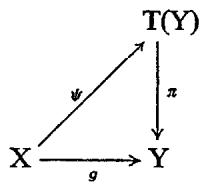
\includegraphics[keepaspectratio]{images/part001_bb2423ff.jpg}}

交换，其中 \(\pi\) 表示 T(Y) 到 Y 的典范投影。给定 \(\psi\) 等价于给定向量丛 \(g^{*}\mathrm{T}(\mathrm{Y})\) 的一个截面，即 T(Y) 在 g 下的逆像的一个截面。

提升的概念推广了向量场的概念（当 \(g = \operatorname{Id}_{\mathbf{X}}\) 时退化为向量场）；关于 \(\theta_{\xi}\) 和 \(i(\xi)\) 的定义与结果的重要部分也推广到提升；我们只简要指出其中几项。

8.6.2. 设 \(\psi: X \to T(Y)\) 是 \(g: X \to Y\) 的一个提升，并设 \(\omega\) 是一个 \(p\) 次、定义在 \(Y\) 上、取值于向量丛 \(F\)（其基底为 \(Y\)）的微分形式。当 \(p \geqslant 1\) 时，将微分形式 \(i(\psi,\omega)\)、或 \(i(\psi)\omega\)、或 \(i_{\psi}(\omega)\) 记在 X 上；它们的次数为 \(p-1\)，取值于 \(g^{*}\mathbf{F}\)，并满足

\[
i (\psi , \omega) _ {x} (v _ {1}, \dots , v _ {p - 1}) = \omega_ {g (x)} (\psi (x), T _ {x} (g). v _ {1}, \dots , T _ {x} (g). v _ {p - 1})\tag{1}
\]

对所有 \(x \in X\) 以及每个 \(v_1, \ldots, v_{p-1}\)（其元素属于 \(\mathbf{T}_x(X)\)），上述关系都成立。当 \(p = 0\) 时，令 \(i(\psi, \omega) = 0\)。称 \(i(\psi, \omega)\) 为 \(\psi\) 与 \(\omega\) 的内积；若 \(\psi\) 和 \(\omega\) 属于 \(\mathbf{C}^r\) 类，则 \(i(\psi, \omega)\) 也属于该类。设 \(\mathbf{F}' \times_{\mathbb{Y}} \mathbf{F}'' \to \mathbf{F}\) 是以 Y 为基底的向量丛的一个配对。对于 \(\omega' \in {}^\tau \Omega^{p'}(Y; F')\) 和 \(\omega'' \in {}^\tau \Omega^{p''}(Y; F'')\)，有

\[
i (\psi) \left(\omega^ {\prime} \wedge \omega^ {\prime \prime}\right) = (i (\psi) \omega^ {\prime}) \wedge g ^ {*} \omega^ {\prime \prime} + (- 1) ^ {p ^ {\prime}} g ^ {*} \omega^ {\prime} \wedge i (\psi) \omega^ {\prime \prime}.\tag{2}
\]

8.6.3. 例子

\begin{enumerate}
\def\labelenumi{\alph{enumi})}
\tightlist
\item
  X 上的向量场 \(\xi\) 定义了 g 在 T(Y) 中的提升 T(g) \(\circ\) \(\xi\)，并且有：
\end{enumerate}

\[
i (\mathrm{T} (g) \circ \xi) = i (\xi) \circ g ^ {*}.\tag{3}
\]

\begin{enumerate}
\def\labelenumi{\alph{enumi})}
\setcounter{enumi}{1}
\tightlist
\item
  Y 上的向量场 \(\eta\) 定义了 \(\eta \circ g\) 在 T(Y) 中的提升 \(g\)，并且有：
\end{enumerate}

\[
i (\eta \circ g) = g ^ {*} \circ i (\eta).\tag{4}
\]

\begin{enumerate}
\def\labelenumi{\alph{enumi})}
\setcounter{enumi}{2}
\tightlist
\item
  更一般地，设 \(h: \mathbf{Y} \to \mathbf{Z}\) 是 \(\mathbf{C}^{r+1}\) 类流形的态射。若 \(\psi\) 是 \(g\) 到 \(\mathbf{T}(\mathbf{Y})\) 的提升，则 \(\mathbf{T}(h) \circ \psi\) 是 \(h \circ g\) 到 \(\mathbf{T}(\mathbf{Z})\) 的提升，并且有：
\end{enumerate}

\[
i (\mathrm{T} (h) \circ \psi) = i (\psi) \circ h ^ {*}.\tag{5}
\]

若 \(\varphi\) 是 \(h\) 到 \(\mathrm{T}(Z)\) 的提升，则 \(\varphi \circ g\) 是 \(h \circ g\) 到 \(\mathrm{T}(Z)\) 的提升，并且有：

\[
i (\varphi \circ g) = g ^ {*} \circ i (\varphi).\tag{6}
\]

8.6.4（“无穷小变换”）。设 \(\psi\) 是 \(C^r\) 类的 \(g\) 的提升，且 \(\omega\) 是 Y 上取值于 Banach 空间 F、次数为 \(p\) 且属于 \(C^r\) 类的微分形式。X 上的微分形式

\[
d (i (\psi) \omega) + i (\psi) d \omega\tag{7}
\]

是次数为 \(p\) 的 \(\mathbf{C}^{r-1}\) 类形式；记为 \(\theta_{\psi}.\omega\)。

若 f 是 X 上的 \(C^{r}\) 类函数，则有

\[
\theta_ {f \psi}. \omega = d f \wedge i (\psi) \omega + f \theta_ {\psi}. \omega .\tag{8}
\]

8.6.5（“将 \(\theta_{\psi}.\omega\) 刻画为导数”）。保持 8.6.4 的假设。设 \(x\in X\)。则存在 \(x\) 的一个开邻域 U、K 中 0 的一个开邻域 I，以及一个 \(C^{r}\) 类态射 G: I × U → Y，具有下列两个性质：

\begin{enumerate}
\def\labelenumi{\alph{enumi})}
\item
  对每个 \(x \in \mathbf{U}\)，有 \(\mathbf{G}(0, x) = g(x)\)。
\item
  对每个 \(x \in \mathbf{U}\)，切向量 (1, 0) 在 \(\mathrm{T}_{(0,x)}(\mathrm{G})\) 下的像等于 \(\psi(x)\)。
\end{enumerate}

设 (U, I, G) 满足这些条件；对于每个 \(t \in \mathbf{I}\)，记从 U 到 Y 的映射 \(\mathbf{G}_t\) 为 \(x \mapsto \mathbf{G}(t, x)\)；置 \(\omega_t = \mathbf{G}_t^*(\omega)\)。对于每个 \(x \in \mathbf{X}\)，从 I 到 \(t \mapsto \omega_t(x)\) 的映射 \(\operatorname{Alt}^p(\mathrm{T}_x(\mathbf{X}), \mathbf{F})\) 属于 \(\mathbf{C}^r\) 类，且其在原点处的导数由下式给出

\[
\frac {d}{d t} (\omega_ {t} (x)) _ {t = 0} = (\theta_ {\psi}. \omega) (x).\tag{9}
\]

